\ylDisplay{Langev takisti} % Ülesande nimi
{Tundmatu autor} % Autor
{piirkonnavoor} % Voor
{2011} % Aasta
{G 8} % Ülesande nr.
{6} % Raskustase
{
% Teema: Magnetism
\ifStatement
\begin{wrapfigure}{r}{0.2\textwidth}
	\vspace{-20pt}	
	\begin{center}
		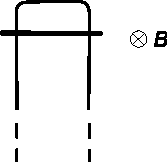
\includegraphics[width=0.9\linewidth]{2011-v2g-08-yl}
	\end{center}
	\vspace{-20pt}
\end{wrapfigure}

Joonisel kujutatud Maa gravitatsiooniväljas vertikaalselt paiknevale juhtivale traadile kinnitati takisti nõndaviisi, et see võib piki traati vabalt libiseda. Teades, et magnetinduktsioon oli $B$ ja traadi harude vaheline kaugus $d$, leidke, millise lõppkiirusega hakkab takisti langema. Takisti mass on $m$ ja takistus $R$.
\fi


\ifHint
Raamis indutseeritakse vool, sest takisti kukkudes suureneb raami läbiv magnetvoog, mis omakorda tekitab Faraday seaduse kohaselt raamis elektromotoorjõu ja voolu. Seega on stabiilses režiimis raskusjõud ning takistit läbiva voolu poolt tekitatud Lorentzi jõud tasakaalus.
\fi


\ifSolution
Raami läbiva magnetvoo suuruse muutus põhjustab raamis elektromotoorjõu $\mathcal{E} = \D\Phi/\D t = Blv$. Elektromotoorjõud põhjustab raamis voolu $I = \mathcal{E}/R$. Magnetväljas mõjub vooluga juhtmele jõud $F = BIl$, mis peab olema tasakaalus raskusjõuga $mg$. Elimineerides $I$ ja $\mathcal{E}$ leiame
\[
m g=\frac{B^{2} l^{2} v}{R} \Rightarrow v=\frac{m g R}{B^{2} d^{2}}.
\]

\medskip

\emph{Alternatiivne lahendus}

Lahendus lähtub energia jäävuse seadusest. Gravitatsioonijõu poolt tehtud töö võimsus on $P = mgv$. Elektrilise töö võimsus peab sellega võrduma, seega $P = mgv = U^2/R$. Pinge on leitav Faraday seadusest, mille kohaselt on pinge võrdne kontuuri läbiva magnetvoo muutumise kiirusega. Magnetvoo muutumise kiirus on $\D\Phi/\D t = Bd v$. Asendades selle eelmisesse võrrandisse ja avaldades $v$ saame 
\[
v=\frac{m g R}{B^{2} d^{2}}.
\] 
\fi
}